%============================ MANUALES (ENTREGA 3) ==========================
\chapter{Manuales de usuario y técnico}
\label{cap:manuales}

\section{Manual de usuario}
El recorrido visual completo de la plataforma ---con capturas de cada sección--- se
presenta en el Capítulo~\ref{cap:plataforma}. Esta sección resume el uso operativo.

\subsection{Requisitos previos y preparación}
Antes de iniciar una sesión se debe disponer de la placa ESP32 con la pantalla OLED
y el pulsador conectados, una fuente USB estable y un equipo con navegador moderno.
Para la primera puesta en marcha se recomienda utilizar el cable USB del computador;
para operación autónoma se utiliza el portapilas con salida USB regulada descrito en
el Capítulo~\ref{cap:electronica}. No se deben conectar simultáneamente ambas fuentes.
El operador debe comprobar que la antena de la placa no quede cubierta por metal y
que el pulsador pueda accionarse sin abrir la carcasa.

\subsection{Secuencia de arranque del ESP32}
La secuencia normal de uso es la siguiente:
\begin{enumerate}[leftmargin=1.8em]
  \item Conectar una única fuente de alimentación y esperar el mensaje inicial en la OLED.
  \item El ESP32 intenta asociarse a la red Wi\nobreakdash-Fi configurada y abre el WebSocket seguro con el servidor.
  \item Confirmar en la cabecera del dashboard que el dispositivo figura como \emph{En línea}; en la OLED debe aparecer \code{[WS:OK]}.
  \item Seleccionar el modo desde el dashboard o pulsar brevemente el botón para avanzar al siguiente modo.
  \item Mantener el dispositivo en una ubicación despejada, evitando acercarlo a routers o fuentes de ruido si se desea una medición representativa.
\end{enumerate}

\begin{figure}[H]
\centering
\fcolorbox{gray!45}{white}{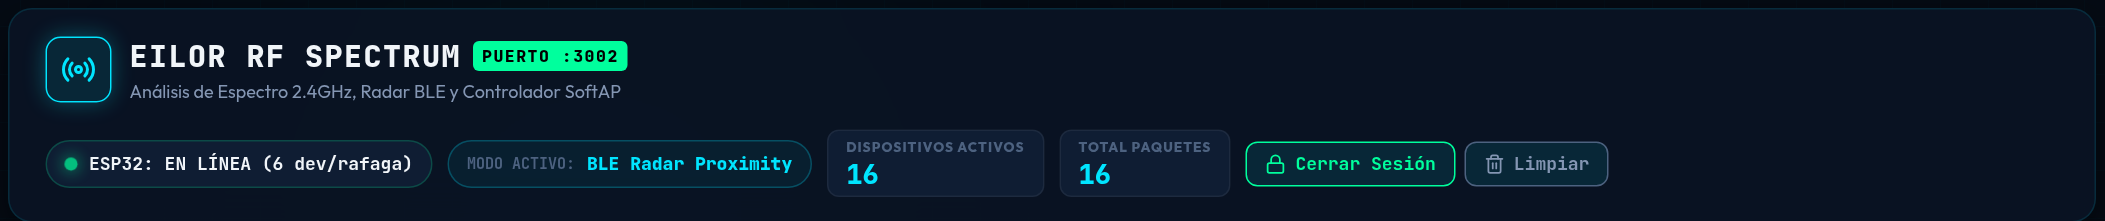
\includegraphics[width=0.95\linewidth]{figuras/cap-cabecera}}
\caption{Indicadores de operación: conexión del ESP32, modo activo y contadores globales.}
\label{fig:manual-cabecera}
\end{figure}

\subsection{Acceso al dashboard}
El tablero de mando se abre desde un navegador en la dirección publicada (por ejemplo, \plataformaurl) o localmente en \code{http://localhost:3002}. La interfaz muestra, en tiempo real, el estado del ESP32, el modo activo y los contadores de dispositivos y paquetes.

\subsection{Inicio de sesión}
Para ejecutar acciones de control (cambiar de modo, desplegar SoftAP, limpiar datos o ver registros) se requiere iniciar sesión con el botón \emph{Iniciar Sesión} e introducir la contraseña configurada. Sin sesión, el sistema opera en modo de solo lectura.

\subsection{Modos del dispositivo}
Los cuatro modos se conmutan desde el panel de control o con el pulsador físico: (0)~Espectro Wi\nobreakdash-Fi, (1)~Radar BLE, (2)~SoftAP con portal cautivo y (3)~Standby.

\begin{description}[leftmargin=2.6cm,style=nextline]
  \item[Modo 0 --- Espectro Wi\nobreakdash-Fi.] Recorre los canales 1--13 y muestra el total de redes, el canal más saturado y una recomendación. Es el modo apropiado para diagnosticar interferencia de acceso.
  \item[Modo 1 --- Radar BLE.] Escucha las balizas de advertising y resume cantidad, nombre visible y RSSI del dispositivo más cercano. La ausencia de nombre no implica ausencia de dispositivo.
  \item[Modo 2 --- SoftAP.] Crea la red propia de invitados y atiende el portal cautivo. Solo debe emplearse en redes autorizadas y con un SSID claramente identificable.
  \item[Modo 3 --- Standby/telemetría.] Mantiene el enlace y envía estado, dirección IP y telemetría sin iniciar un ciclo de escaneo intensivo.
\end{description}

\begin{figure}[H]
\centering
\fcolorbox{gray!45}{white}{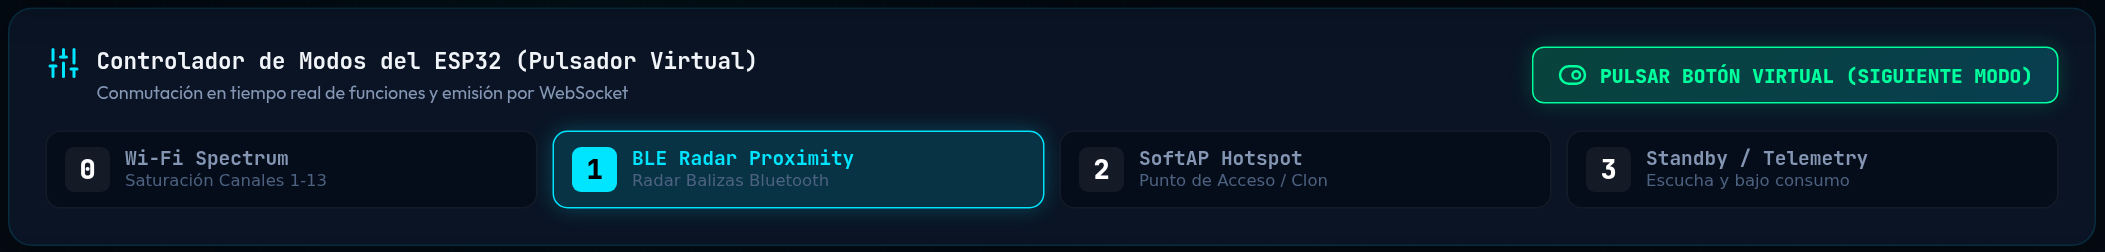
\includegraphics[width=0.95\linewidth]{figuras/cap-modos}}
\caption{Selector de los cuatro modos disponibles para el ESP32.}
\label{fig:manual-modos}
\end{figure}

En el modo Wi\nobreakdash-Fi conviene esperar al menos un ciclo completo antes de
interpretar la gráfica. En el radar BLE se deben comparar varias muestras porque
el RSSI cambia con la orientación y el movimiento. El botón físico usa lógica
activa en bajo: cada pulsación válida cambia de modo y el antirrebote evita cambios
duplicados.

\subsection{Lectura de espectro y radar}
La vista de espectro permite localizar canales con mayor ocupación y comparar la
distribución de puntos de acceso. La recomendación de canal es una ayuda heurística,
no una garantía de rendimiento: debe contrastarse con el ancho de canal y la
ubicación física del router. La vista radar muestra dispositivos BLE detectados,
su RSSI y la última actualización recibida.

\begin{figure}[H]
\centering
\fcolorbox{gray!45}{white}{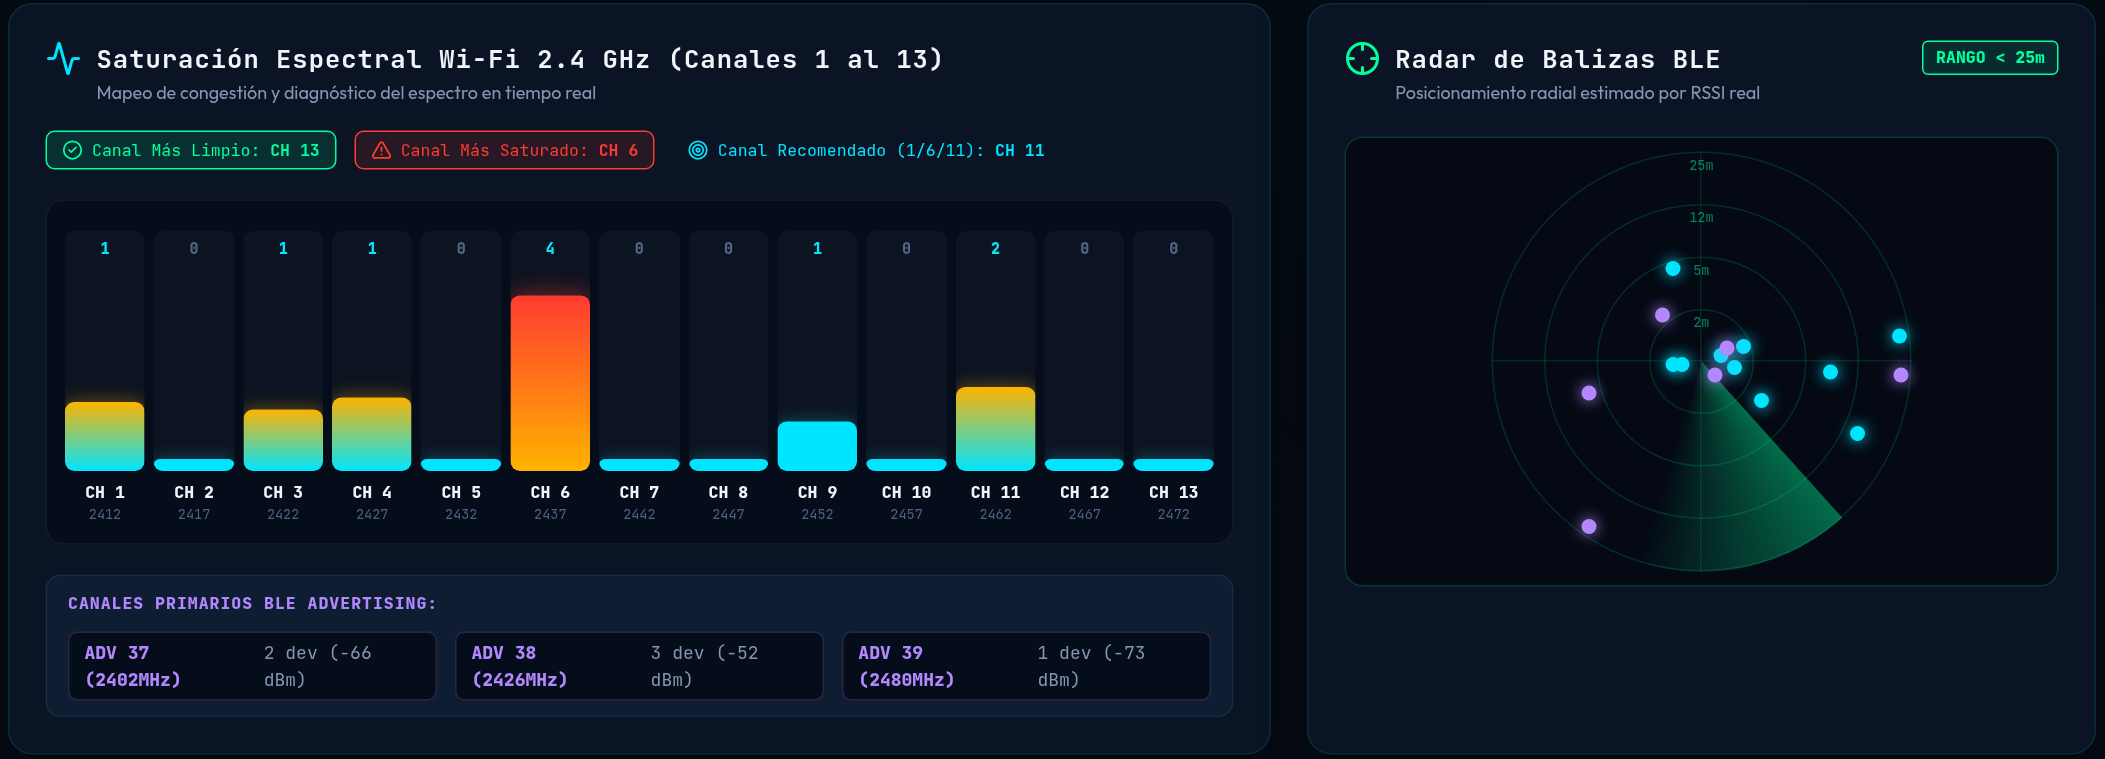
\includegraphics[width=0.98\linewidth]{figuras/cap-espectro-radar}}
\caption{Uso del mapa de saturación Wi\nobreakdash-Fi y del radar BLE para observar el entorno de 2.4~GHz.}
\label{fig:manual-espectro}
\end{figure}

\subsection{Despliegue del punto de acceso y portal}
En la sección SoftAP se define el SSID y el canal, y se pulsa \emph{Desplegar SoftAP}. Al conectarse un invitado a esa red, aparece automáticamente el portal cautivo con el formulario de registro.

El procedimiento recomendado es: (1) iniciar sesión; (2) escribir un SSID propio,
identificable y autorizado; (3) elegir un canal; (4) pulsar \emph{Desplegar SoftAP};
(5) verificar en la OLED la IP, el SSID y el número de clientes; y (6) probar el
portal desde un teléfono de prueba. Si el sistema operativo no abre la ventana
automática, se puede navegar a \code{http://192.168.4.1}. El portal no debe usarse
para imitar redes de terceros ni para capturar datos sin consentimiento.

\begin{figure}[H]
\centering
\fcolorbox{gray!45}{white}{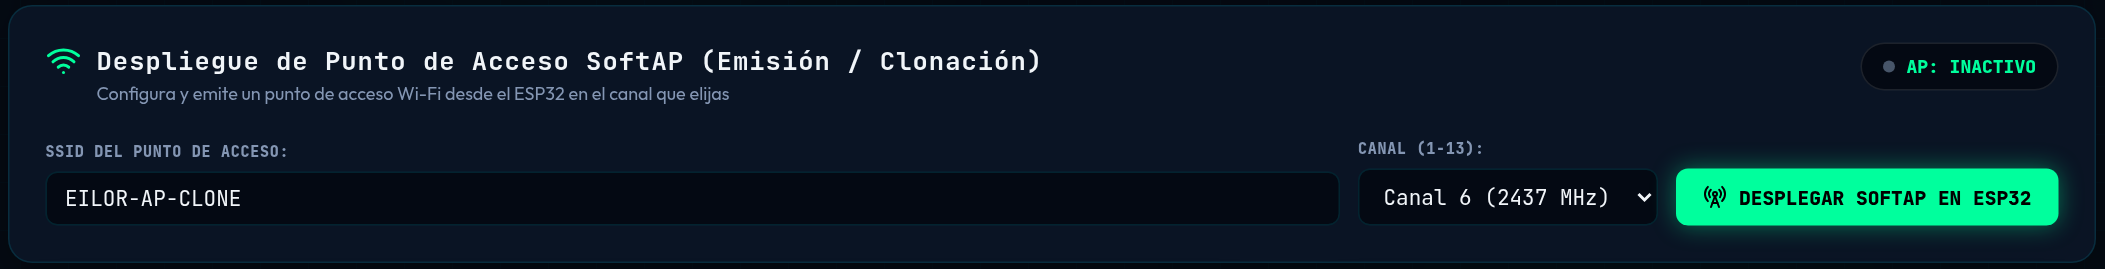
\includegraphics[width=0.78\linewidth]{figuras/cap-softap}}
\caption{Configuración del SoftAP: SSID, canal y activación controlada desde el dashboard.}
\label{fig:manual-softap}
\end{figure}

\begin{figure}[H]
\centering
\fcolorbox{gray!45}{white}{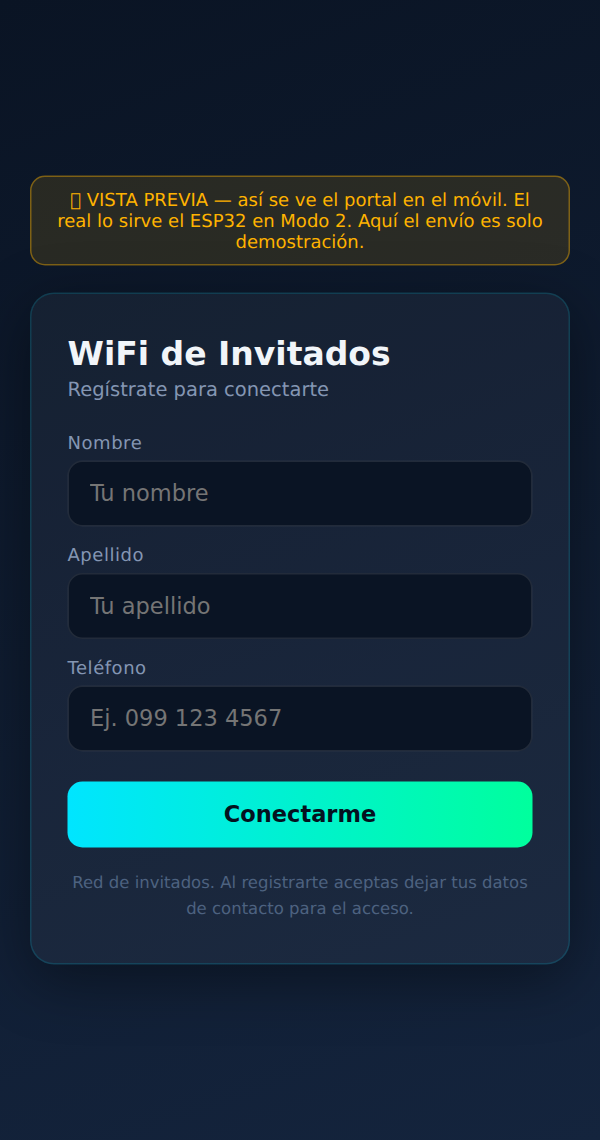
\includegraphics[height=7.2cm]{figuras/cap-portal}}
\caption{Portal cautivo que visualiza el invitado al conectarse a la red propia.}
\label{fig:manual-portal}
\end{figure}

\subsection{Registros de invitados}
La sección \emph{Registros del Portal Cautivo} lista las altas (nombre, apellido, teléfono, red y fecha) en tiempo real. Desde allí se puede \emph{Exportar CSV} o \emph{Borrar} los registros (ambas acciones requieren sesión).

Antes de exportar, el operador debe verificar que la captura fue informada y
consentida. El archivo CSV debe almacenarse con permisos restringidos y eliminarse
cuando finalice el periodo de retención definido por la organización. La acción
\emph{Borrar} es irreversible desde la interfaz, por lo que se recomienda exportar
solo cuando exista una finalidad legítima y una copia controlada.

\begin{figure}[H]
\centering
\fcolorbox{gray!45}{white}{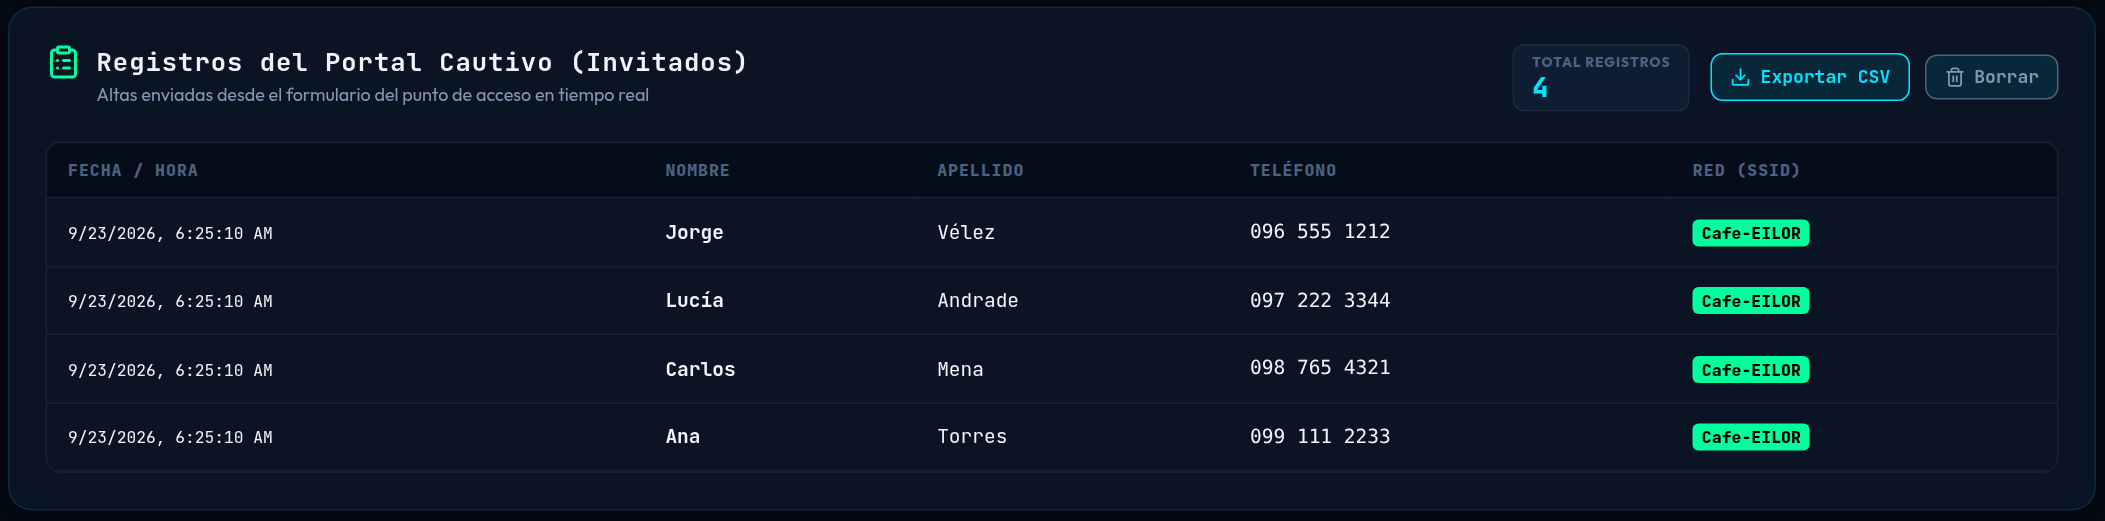
\includegraphics[width=0.95\linewidth]{figuras/cap-registros}}
\caption{Registros del portal cautivo y controles de exportación y limpieza.}
\label{fig:manual-registros}
\end{figure}

\subsection{Indicadores y telemetría}
La tarjeta de telemetría confirma la última muestra, el estado del enlace y la
actividad del dispositivo. Una demora aislada no implica una falla: primero se
debe observar si el contador se actualiza después del siguiente heartbeat. La
vista de dispositivos ayuda a distinguir redes detectadas, balizas BLE y registros
del portal; no debe interpretarse como una captura del contenido de las comunicaciones.

\begin{figure}[H]
\centering
\fcolorbox{gray!45}{white}{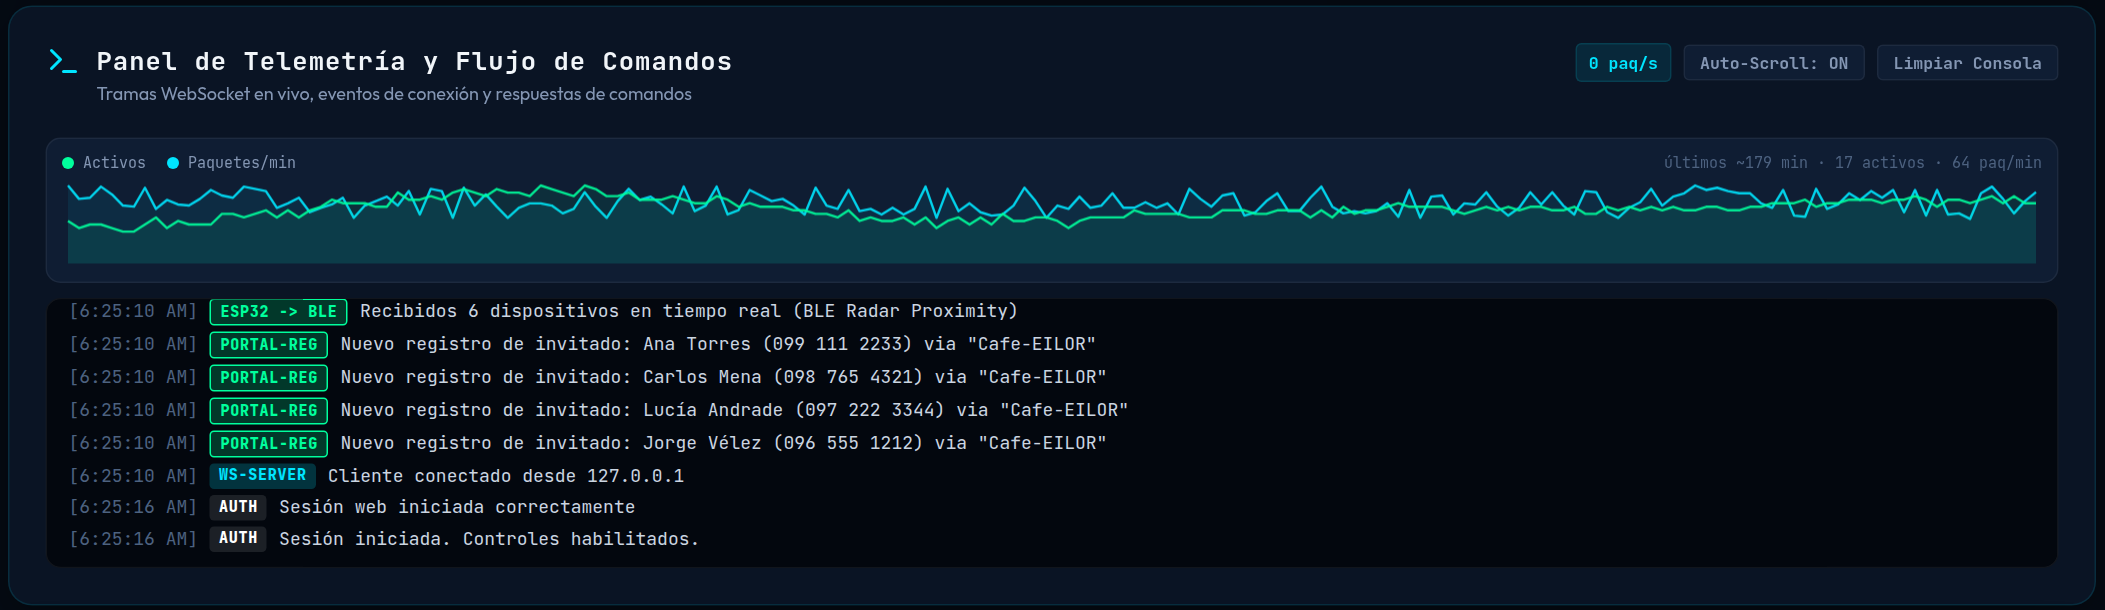
\includegraphics[width=0.95\linewidth]{figuras/cap-telemetria}}
\caption{Panel de telemetría y estado de la conexión del dispositivo.}
\label{fig:manual-telemetria}
\end{figure}

\captura[0.62]{cap-dashboard-full}{Vista completa del \emph{dashboard} con todas sus secciones (cabecera, controlador de modos, SoftAP, espectro, radar, telemetría, inventario y registros).}

\section{Manual técnico}
\subsection{Flujo técnico de extremo a extremo}
El firmware inicia Wi\nobreakdash-Fi en modo estación, configura I\textsuperscript{2}C
en GPIO21/GPIO22, inicializa la OLED en la dirección 0x3C y registra el pulsador
en GPIO15 con \code{INPUT\_PULLUP}. Después establece el WebSocket TLS hacia el
servidor. Cada ciclo de escaneo produce un mensaje JSON con tipo de medición,
modo, identificador de dispositivo y resultados; el servidor valida, persiste y
difunde la actualización a los navegadores conectados.

\begin{figure}[H]
\centering
\fcolorbox{gray!45}{white}{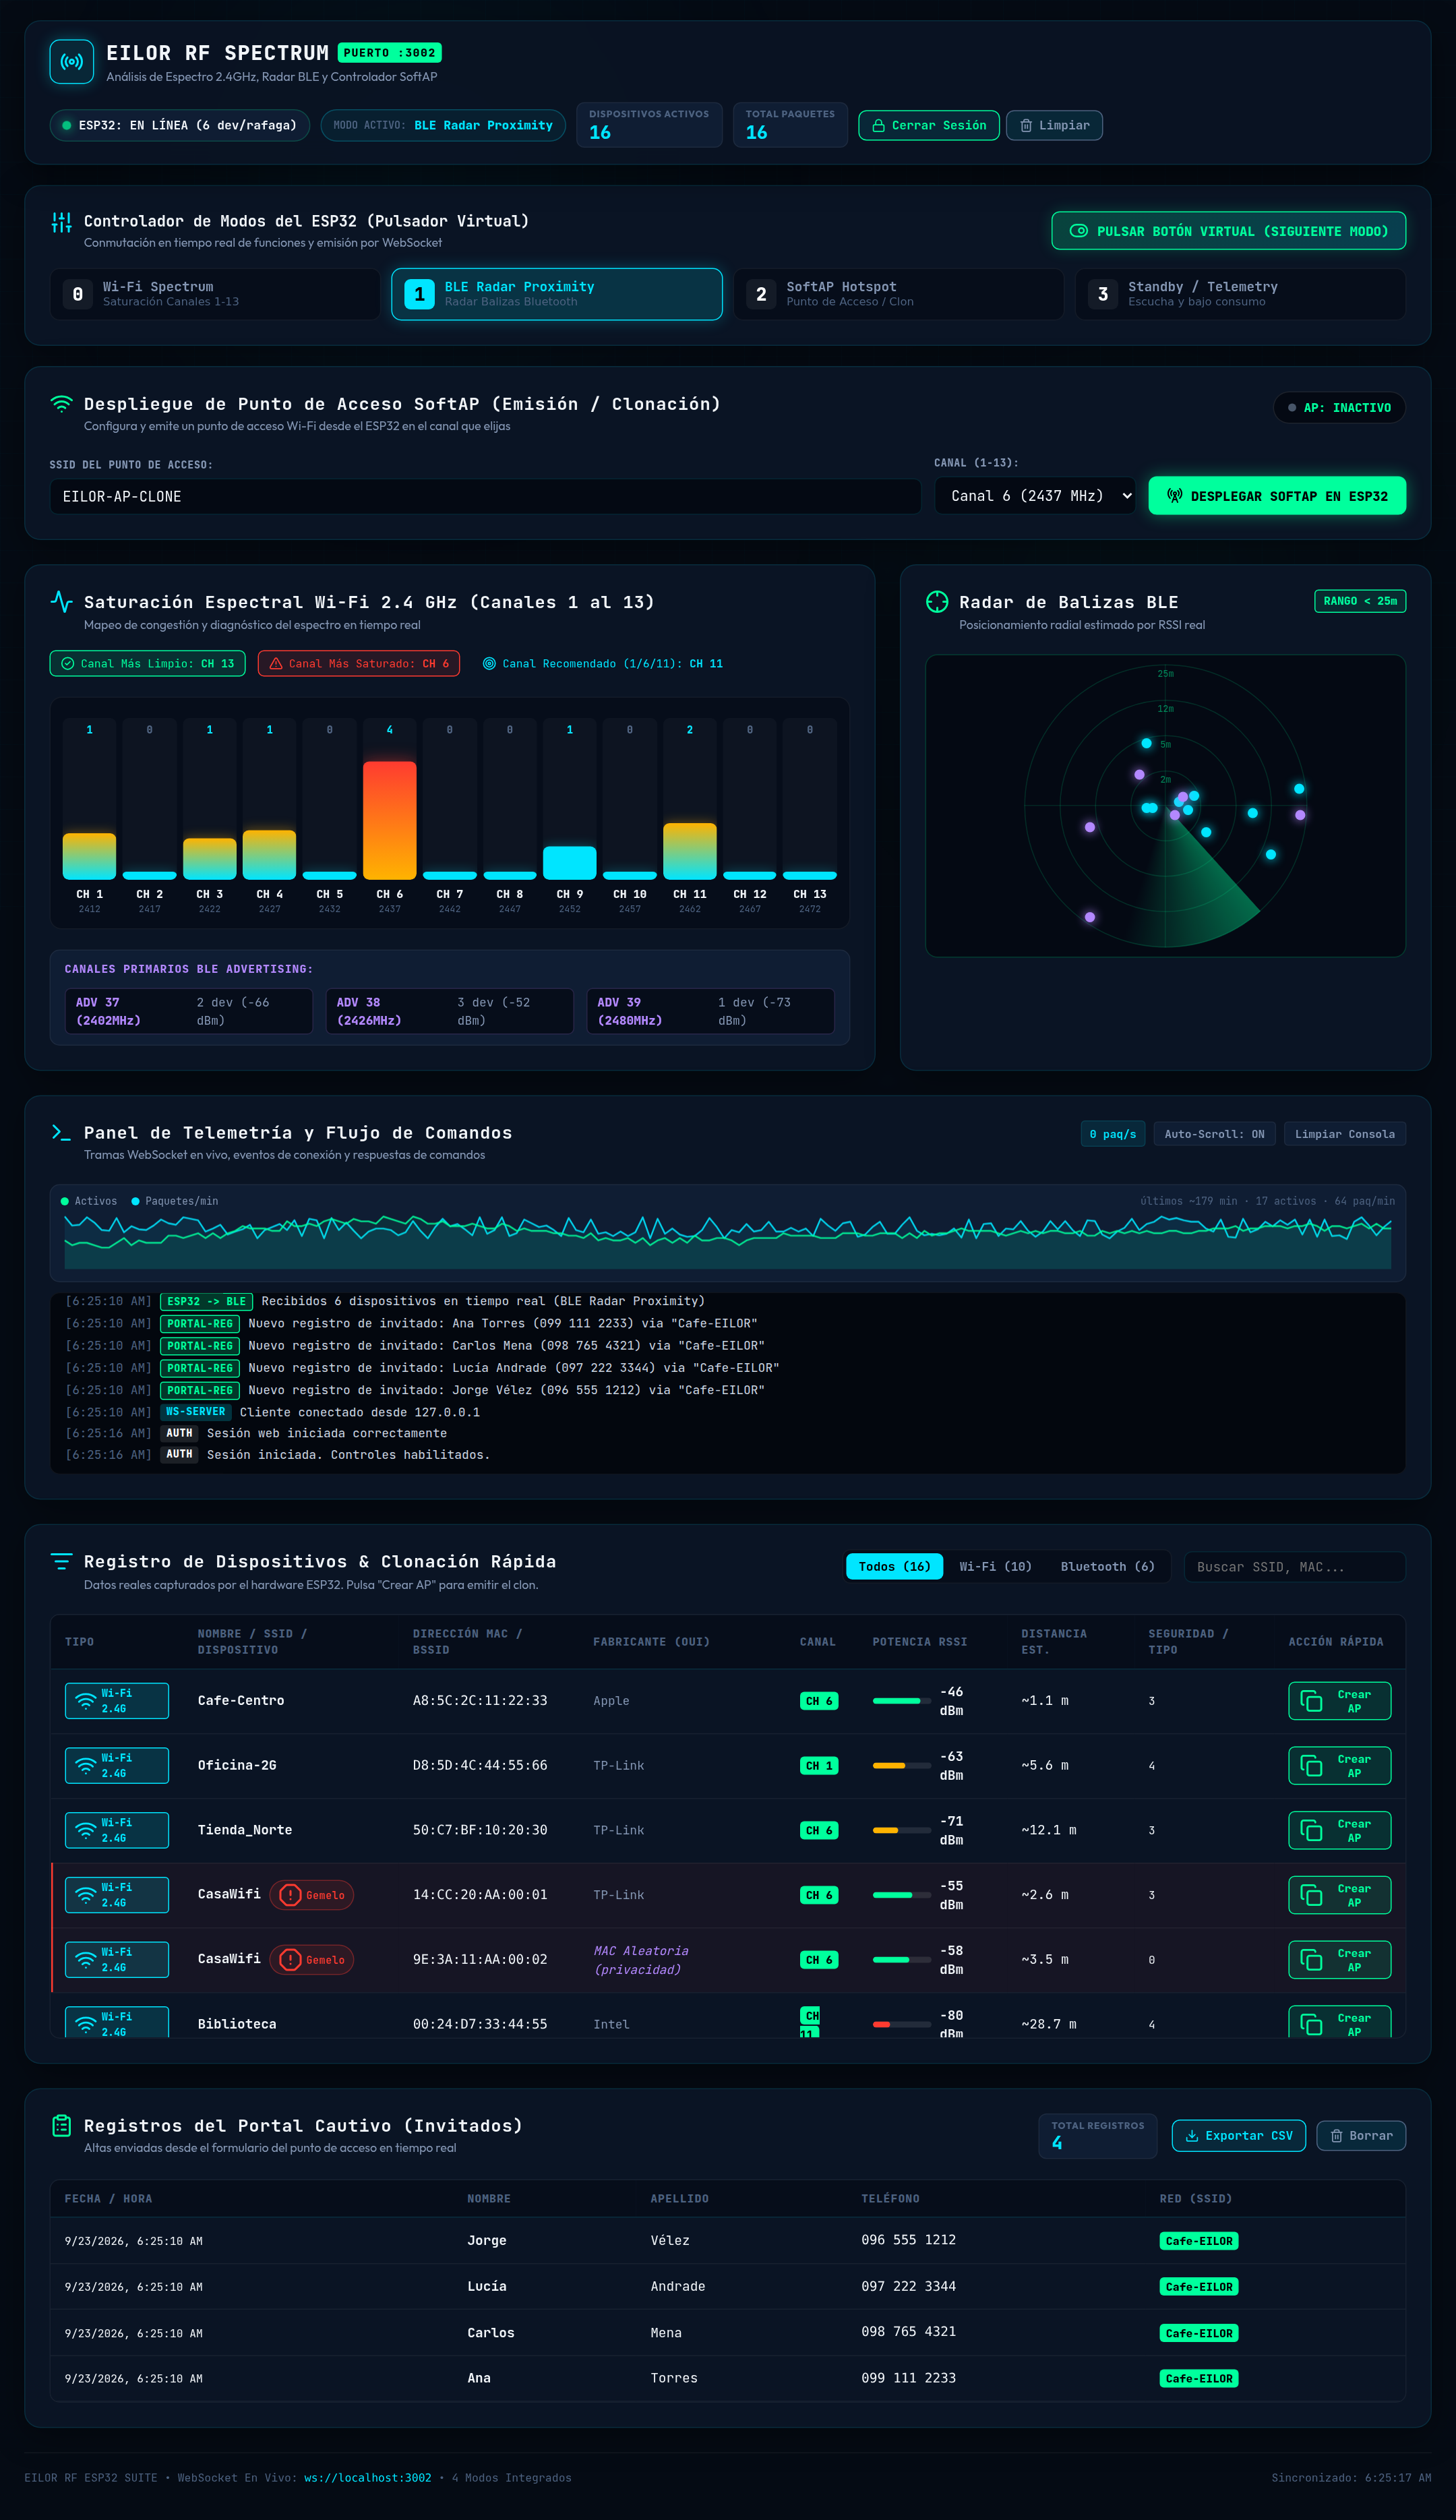
\includegraphics[width=0.98\linewidth]{figuras/cap-dashboard-full}}
\caption{Vista de referencia para validar el flujo completo después de una instalación técnica.}
\label{fig:manual-flujo}
\end{figure}
\subsection{Estructura del proyecto}
\begin{lstlisting}[style=bash,caption={Estructura de directorios},basicstyle=\ttfamily\footnotesize]
eilor/
  server.js              # servidor Express + WebSocket
  lib/                   # modulos: analysis, oui, store, auth
  public/                # dashboard: index.html, app.js, styles.css, portal-preview.html
  firmware/              # eilor_esp32.ino (firmware del ESP32)
  data/                  # persistencia JSON (se crea sola; en .gitignore)
  package.json
\end{lstlisting}

\subsection{Instalación y ejecución del servidor}
\begin{lstlisting}[style=bash,caption={Puesta en marcha del servidor},basicstyle=\ttfamily\footnotesize]
cd eilor
npm install                       # instala express, ws, cors
EILOR_PASSWORD="tu_clave" node server.js
# o gestionado con PM2:
pm2 start server.js --name eilor && pm2 save
\end{lstlisting}

\subsection{Variables de entorno}
\begin{table}[H]
\centering
\caption{Variables de entorno del servidor}
\label{tab:env}
\footnotesize
\begin{tabularx}{\linewidth}{@{}l X l@{}}
\toprule
\textbf{Variable} & \textbf{Función} & \textbf{Valor por defecto} \\
\midrule
\code{PORT} & Puerto de escucha & 3002 \\
\code{HOST} & Interfaz de escucha & 127.0.0.1 \\
\code{EILOR\_PASSWORD} & Contraseña del dashboard & Obligatoria; sin valor por defecto \\
\code{EILOR\_DEVICE\_TOKEN} & Token para restringir la ingesta & (sin definir: ingesta abierta) \\
\bottomrule
\end{tabularx}
\end{table}

\subsection{Carga del firmware}
El firmware se compila y sube desde Arduino IDE o PlatformIO. Debe ubicarse en una carpeta con su mismo nombre. Antes de compilar se configuran las credenciales Wi\nobreakdash-Fi, el \code{WS\_SERVER\_HOST} y, opcionalmente, el \code{DEVICE\_TOKEN} y el nombre del portal (\code{PORTAL\_TITULO}). Librerías requeridas: \code{WebSockets} (Markus Sattler), \code{Adafruit\_SSD1306}, \code{Adafruit\_GFX} y \code{ezButton}.

Después de cargar el firmware, abrir el monitor serie a 115200~baudios y comprobar,
en orden, la inicialización de la OLED, la asociación Wi\nobreakdash-Fi, la conexión
TLS y los mensajes de cambio de modo. Si la pantalla no inicia, comprobar VCC,
GND, SDA, SCL y la dirección I\textsuperscript{2}C antes de volver a grabar. Para
actualizar varias unidades se debe conservar el mismo identificador lógico del
dispositivo únicamente cuando cada unidad tenga su propio token y registro de
inventario.

\subsection{Prueba técnica de aceptación}
La siguiente lista permite cerrar una instalación con evidencia reproducible:
\begin{enumerate}[leftmargin=1.8em]
  \item El servidor inicia sin errores y responde en el puerto configurado.
  \item El dashboard permite iniciar sesión y cambia a solo lectura cuando se cierra sesión.
  \item El ESP32 aparece en línea y envía al menos un heartbeat.
  \item El modo Wi\nobreakdash-Fi actualiza redes y el radar BLE actualiza dispositivos.
  \item El botón cambia entre los cuatro modos sin rebotes visibles.
  \item El SoftAP entrega una IP, muestra clientes en la OLED y presenta el portal.
  \item Un registro sin conexión queda en cola y se reenvía al recuperar el WebSocket.
  \item La exportación CSV y la limpieza solo funcionan con sesión autenticada.
\end{enumerate}

La evidencia mínima debe incluir una captura de la cabecera, una del modo de
escaneo, una del portal y una del registro recibido. Estas imágenes se conservan
junto con la fecha, versión del firmware y configuración del servidor.

\subsection{Publicación con Cloudflare Tunnel}
\begin{lstlisting}[style=bash,caption={Publicación del servicio con cloudflared},basicstyle=\ttfamily\footnotesize]
cloudflared tunnel create eilor-tunnel
cloudflared tunnel route dns eilor-tunnel esp.tu-dominio.com
cloudflared tunnel run eilor-tunnel   # usa el config.yml del Cap. 8
\end{lstlisting}

\subsection{Resolución de problemas frecuentes}
\begin{itemize}[leftmargin=1.4em]
  \item \textbf{OLED apagada o con basura:} comprobar 3V3/GND, invertir SDA/SCL solo si el módulo lo exige y verificar la dirección 0x3C.
  \item \textbf{ESP32 reinicia al escanear:} sustituir el cable o fuente por una capaz de entregar al menos 500~mA y comprobar que no se estén usando dos fuentes.
  \item \textbf{ESP32 marca "sin conexión":} verificar credenciales Wi\nobreakdash-Fi, hora del sistema, alcance del túnel y que el servidor esté en línea (\code{pm2 logs eilor}).
  \item \textbf{El botón cambia dos modos:} revisar el cable entre GPIO15 y GND y mantener el antirrebote de 50~ms del firmware.
  \item \textbf{El portal no aparece:} confirmar que el dispositivo está en modo 2 y abrir \code{http://192.168.4.1}.
  \item \textbf{Registros no llegan:} revisar el enlace WebSocket y el contador de clientes; el \emph{buffer} reenviará al reconectar mientras no se alcance su capacidad.
  \item \textbf{Ingesta rechazada (401):} el servidor tiene \code{EILOR\_DEVICE\_TOKEN} definido; configurar el mismo token en el firmware.
  \item \textbf{Dashboard sin datos:} recargar el navegador, confirmar la sesión y revisar que el puerto del servidor coincida con el configurado en el túnel.
\end{itemize}

\subsection{Mantenimiento, respaldo y seguridad}
Antes de modificar firmware o servidor se debe copiar la carpeta \code{data/}, el
archivo de configuración del túnel y la versión actualmente operativa. Las
credenciales Wi\nobreakdash-Fi, la contraseña del dashboard y el token del dispositivo
no deben publicarse en el repositorio. Se recomienda rotarlos cuando cambie el
operador, limitar el acceso al dashboard mediante HTTPS y revisar periódicamente
los registros almacenados. La carcasa debe abrirse con la alimentación desconectada
y las pilas deben retirarse antes de intervenir el cableado.
